\section{Introduction}
\label{sec:introduction}

Language models are increasingly used to generate hypotheses, execute experiments, and evaluate research outputs. End-to-end systems such as the AI Scientist connect these activities into a single pipeline \citep{lu2026towards}. The performance of such a pipeline depends on its research harness: the editable rules, operators, memory, evaluation logic, and stopping conditions that shape what the model does next. A harness can improve without any change to the underlying language model, but demonstrating that improvement requires controls for the proposal space, execution budget, and information available to each condition.

Random legal editing offers a particularly useful reference. If a model-guided process cannot exceed random proposals under the same atomic schema and editable surface, the measured gain may reflect additional search rather than informed adaptation. A fixed initial harness provides a complementary reference by measuring the value of continuation itself. These comparisons become informative only when their champions are evaluated on common support and when failed proposals remain in the end-to-end accounting. Production-scale AutoResearch reports infrastructure fragility, agent memory decay, search-direction stagnation, iteration-cost asymmetry, and metric fixation \citep{chandran2026production}.

This paper asks whether model-guided adaptation improves a complete factor-research process under a fixed model, proposal interface, decision count, and candidate evaluation budget, and whether any effect can be assigned to the information supplied to the proposer. Each model call is asked to return one atomic proposal containing two to five edits. Online execution uses probe information only, while an active branch carries the continuation state and a frozen champion enters one final comparison. Three information conditions vary scalar feedback, cumulative probe memory, and compact diagnostics. Random legal edits and the fixed harness provide matched references across six fresh tasks, two development seeds, and two independent model-call replicates.

The comparison separates quantities that a final score alone would conflate: model calls, expression-candidate positions, and final common support. It also separates end-to-end adaptation from the marginal value of cumulative memory and diagnostics. Failure and call-level variability remain in the process comparison. Novelty and duplicate rate describe select search output, while date-block concentration provides an auxiliary diagnostic for the component contrasts.

The memory-equipped process exceeded both references on the development panel, with median paired gains of 0.003534 over random legal edits and 0.010977 over the fixed harness. The component ablations did not establish stable independent increments from cumulative memory or diagnostics. Median paired differences on the select evaluation showed lower novelty and a higher duplicate rate for memory relative to scalar feedback and random legal edits. These findings support model-guided harness adaptation within the registered setting and show why process evaluation cannot be reduced to a single endpoint.

\section{Related work}
\label{sec:related}

Automated research systems can be compared through the object they adapt, the evidence available during adaptation, and the controls used for final evaluation. The AI Scientist links idea generation, experiment coding and execution, analysis, manuscript writing, and automated review in an end-to-end pipeline \citep{lu2026towards}. Agent Laboratory organizes specialized agents across literature review, experimentation, and report writing, with human feedback available at each stage \citep{schmidgall2025agent}. ARIS combines execution skills and a persistent research wiki with integrity verification, result-to-claim mapping, claim auditing, and reviewer-approved harness improvements \citep{yang2026aris}. AIDE addresses the experimentation layer directly, formulating machine-learning engineering as code optimization through tree search over potential solutions \citep{jiang2025aide}. The present study varies only research-harness decisions, with a frozen factor-expression evaluator and matched proposal controls.

Harness$^2$ provides the closest reference for evidence use during adaptation. Its task-level recursion uses contrastive Propose--Probe--Compose updates, while a second recursion extracts experience from edits for later tasks \citep{xu2026harness2}. SWE-agent shows more generally that agent-computer interface design affects code editing, repository navigation, test execution, and performance \citep{yang2024sweagent}. FunSearch pairs a pretrained model with a systematic evaluator to evolve solution-generating programs \citep{romera2023mathematical}. EoH evolves natural-language heuristic ideas and executable code \citep{liu2024evolution}, and AlphaEvolve extends evaluator-guided evolution to scientific algorithms and computational infrastructure \citep{novikov2025alphaevolve}. GEPA instead reflects on execution traces in natural language to propose and test prompt updates, combining complementary candidates from a Pareto frontier \citep{agrawal2025gepa}. Our continuation adopts the shared principle of feedback-guided adaptation while keeping the factor evaluator fixed. Atomic proposals define complete harness states, random legal edits share the editable surface, and select outcomes remain outside every proposer input.

Evaluation frameworks make different aspects of research performance visible. MLAgentBench measures machine-learning experimentation through file editing, code execution, and output inspection across 13 tasks \citep{huang2023mlagentbench}. MLE-bench covers 75 Kaggle competitions with human leaderboard baselines \citep{chan2024mlebench}. RE-Bench compares agents and human experts in seven open-ended research-engineering environments under varying time budgets \citep{wijk2024rebench}. These designs separate task outcome from the actions, resources, and time required to obtain it.

Scientific-discovery benchmarks add execution and validity requirements. ScienceAgentBench evaluates 102 expert-validated tasks through program quality, execution results, and cost \citep{chen2024scienceagentbench}. DiscoveryWorld provides 120 simulated tasks requiring hypotheses, experiment design and execution, analysis, and conclusions \citep{jansen2024discoveryworld}. AgentBench supplies a broader comparison of reasoning, decision-making, and instruction-following failures across eight interactive environments \citep{liu2023agentbench}. Production-scale AutoResearch complements these benchmarks with observed infrastructure fragility, agent memory decay, search-direction stagnation, iteration-cost asymmetry, and metric fixation \citep{chandran2026production}. Our panel therefore pairs IC contrasts with arm-level call and token accounting, preserved failure records, replicate diagnostics, novelty, and duplicate rate.

Factor-discovery methods define the domain comparison. AlphaGen uses reinforcement learning to optimize a synergistic collection of formulaic alphas through downstream combination-model performance \citep{yu2023generating}. CogAlpha represents alphas as code and combines LLM reasoning with evolutionary mutations, recombination, multi-stage prompts, and financial feedback \citep{liu2025cogalpha}. These methods adapt candidate signals or their collections. Our question concerns the research process that produces those signals: the evaluator and final comparison remain frozen, while the harness, information conditions, and legal-edit reference vary under the registered budget.

\section{Research problem and evidence scope}
\label{sec:problem}

A factor-research harness determines how expression candidates are proposed, evaluated, compared, and retained. Improving that process requires more than increasing the number of formulas produced by a language model. The object of adaptation is the sequence of research decisions, while the object of evaluation is the factor-expression candidate generated under the resulting harness. This study asks whether a language model can improve the former under a fixed protocol, and which sources of information contribute to the measured effect.

Two questions organize the analysis. The first compares a memory-equipped, model-driven process with random legal edits over the same editable surface and with the fixed initial harness. This comparison tests whether model-guided adaptation adds value under matched proposal semantics, decision counts, and candidate evaluation budgets. The second decomposes the model-driven process into scalar feedback, cumulative probe memory, and compact execution diagnostics. It tests whether the additional information channels produce separable improvements over their immediate parent conditions.

All experiments use the development window from 2017-01-01 through 2020-11-30. Task screening and online continuation use probe information only; final select evaluation occurs once after each condition has frozen its champion. The study contains no untouched independent market-period out-of-sample evaluation. Fresh tasks and new development splits within this window provide confirmatory development-panel evidence, and all effect estimates retain that scope.

\section{Research-harness evolution}
\label{sec:harness}

The continuation loop adapts a harness through a bounded sequence of Propose--Probe--Compose decisions. At decision $t$, a proposer receives the current harness and its permitted information packet, then returns one atomic proposal $e_t$ containing two to five edits. The operator $A$ applies the complete array to the current harness and validates the resulting operator roster:
\begin{equation}
H_t^{c}=A(H_{t-1},e_t).
\label{eq:atomic}
\end{equation}
The array therefore represents one composite harness candidate. Earlier JSON arrays with independent-edit semantics retain their historical meaning and are not reinterpreted in the present protocol.

Probe execution evaluates the candidate under the current task contract and produces factor-expression candidates, behavioral measurements, and execution traces. The active branch carries the continuation state into the next decision even when an edit is not adopted. A frozen champion changes only when the task contract is satisfied. This separation allows exploration to continue without turning every temporary improvement into the final evaluated object.

Figure~\ref{fig:method} summarizes the information flow. Historical probe memory excludes select outcomes. Online execution remains probe-only, and one frozen champion per condition enters the final comparison. All relevant candidates and parent signals are evaluated on their common \texttt{date+symbol} support, so paired contrasts do not combine estimates computed on different samples.

\begin{figure*}[!htbp]
\centering
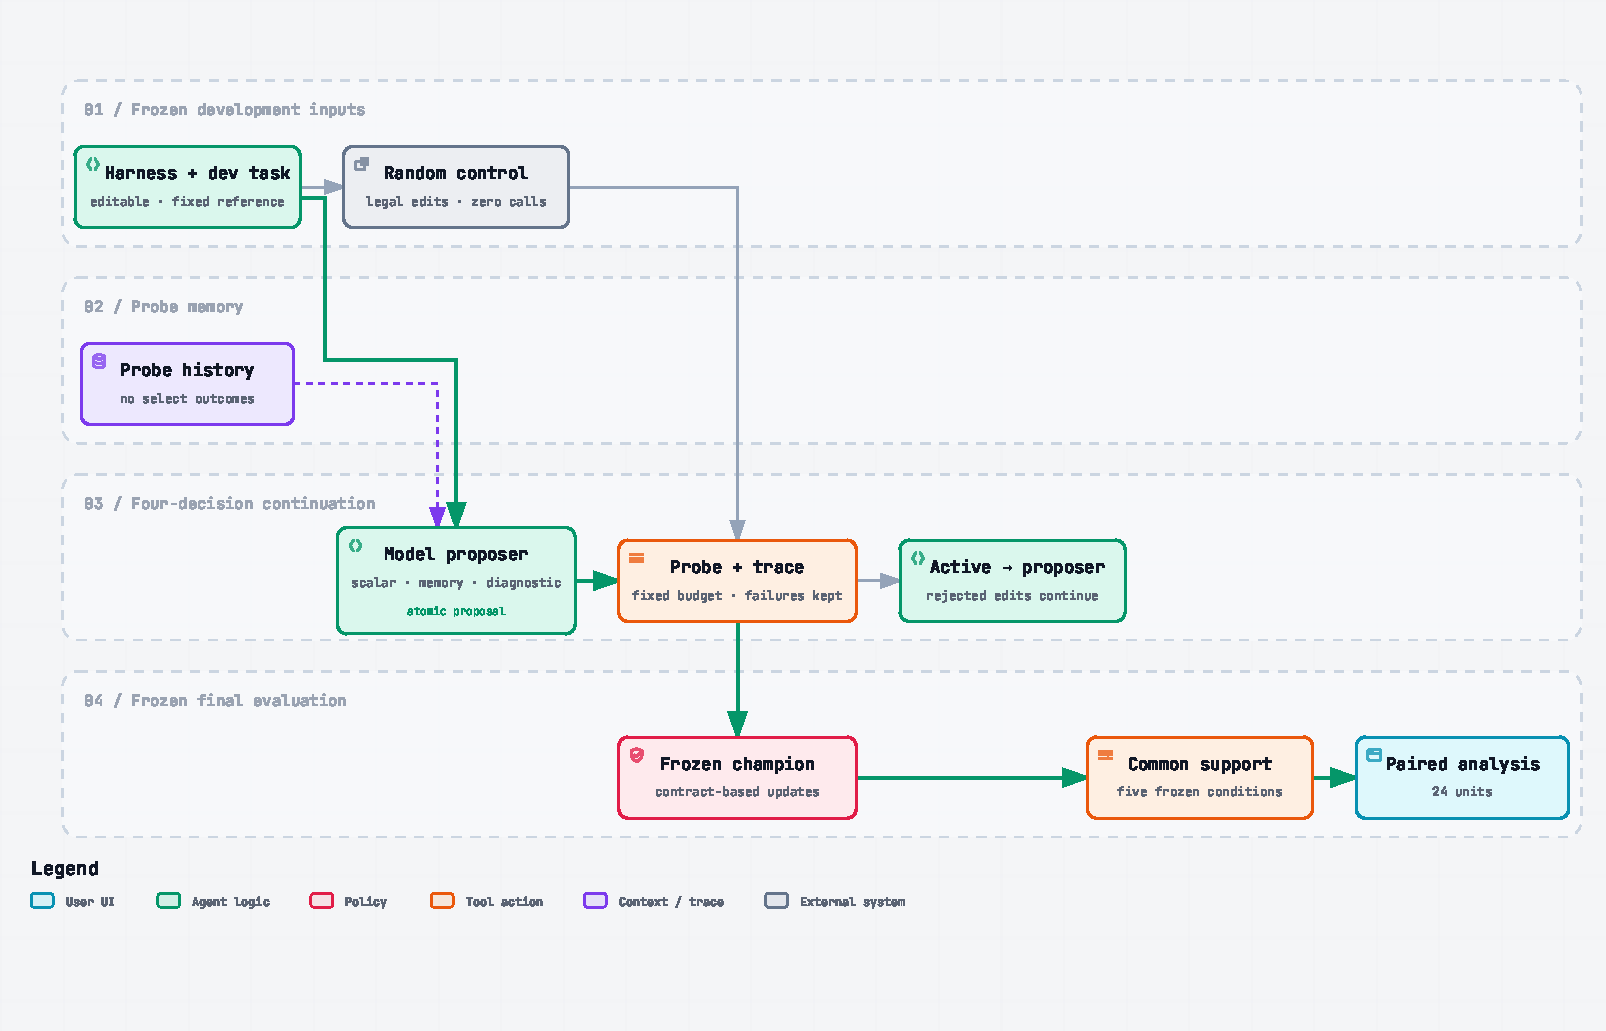
\includegraphics[width=\ResearchWideWidth]{figures/figure_01_method_pipeline.pdf}
\caption{Budget-bounded research-harness continuation and evaluation. Scalar, cumulative-memory, and diagnostic proposers emit one atomic proposal per decision; random legal edits use zero model calls. Probe execution feeds a four-decision active branch and one frozen champion per condition, followed by the final common-support comparison. The diagram also marks the fixed candidate budget, retained failures, and exclusion of select outcomes from historical probe memory.}
\label{fig:method}
\end{figure*}

The random backend reads the same current harness and editable surface and produces legal atomic proposals without a model call. The fixed reference evaluates the unchanged initial harness. These references distinguish model-guided adaptation from random legal edits over the same editable surface and from the initial research process. Within this fixed process, scalar feedback, cumulative memory, and compact diagnostics form the separable information conditions.

\section{Information conditions and controls}
\label{sec:information}

The three model conditions share the model, atomic proposal schema, editable surface, and evaluation protocol. The scalar condition receives the current task, harness, and scalar probe outcomes. The memory condition adds cumulative historical probe memory, including prior failures and behavioral differences that can inform a later decision. The diagnostic condition adds a compact execution trace to that memory, exposing failure categories, mechanism differences, and cost information. Select outcomes remain outside every proposer input.

Two non-model references complete the design. Random legal atomic edits test how much of the observed change can be obtained by sampling the same proposal space with an independent random seed and no language-model calls. The fixed harness measures the unchanged starting process under the same final evaluator. The memory-minus-random contrast is consequently an end-to-end comparison of research processes, whereas memory-minus-scalar and diagnostic-minus-memory isolate incremental information under their respective parent conditions.

Earlier panels played distinct roles in the study design. V001 tested diagnostic continuation and obtained a median paired difference of 0.0, yielding an exploratory development-panel null. V002 tested cumulative memory and obtained a median difference of 0.001224, also yielding an exploratory development-panel null. V003 preserved those records and introduced explicit atomic semantics, a random legal-edit reference, four continuation decisions per arm, six fresh tasks, and independent model-call replicates. These design changes motivate the present panel without converting the earlier exploratory outcomes into confirmatory support.

\section{Paired development-panel protocol}
\label{sec:protocol}

The frozen V003 protocol contains six tasks, T9 through T14, screened with real probe-only execution before the panel. Screening did not run select evaluation. Each task is paired with two development seeds, 11 and 29, and two independent model-call replicates, A and B, producing 24 task--seed--replicate units. A replicate is a separate API call; the provider does not expose a controlled model seed, so replicates measure call-level variability rather than deterministic model-seed effects.

Every model condition receives four continuation decisions and at most twelve factor-expression candidate positions per decision. One model call produces one atomic harness proposal; the candidate positions belong to the subsequent expression evaluation. The random condition follows the same decision schedule and candidate budget with zero model calls. The fixed harness is included in the final common-support comparison for each unit.

Table~\ref{tab:protocol} records the shared design. The proposer is \texttt{kimi/k3.1-pro[1m]} with tools and session persistence disabled and an output ceiling of 8{,}000 tokens per call. Across the complete panel, the protocol permits 288 model calls and 2{,}304{,}000 output tokens. Invalid proposals, empty outputs, and output-limit failures consume their decision and remain in the primary end-to-end analysis.

\begin{table*}[!htbp]
\caption{Frozen V003 development-panel design.}
\label{tab:protocol}
\centering
\ProjectCaption
\small
\begin{tabular}{ll}
\toprule
Design element & Registered value \\
\midrule
Tasks & T9--T14 (six fresh tasks) \\
Development seeds & 11 and 29 \\
Model-call replicates & A and B, independent calls \\
Paired units & 24 \\
Continuation decisions per model arm & 4 \\
Expression-candidate positions per decision & At most 12 \\
Proposal schema & \texttt{AUTO-RESEARCH-ATOMIC-PROPOSAL-1} \\
Model & \texttt{kimi/k3.1-pro[1m]} \\
Maximum model calls & 288 \\
Maximum output tokens & 2{,}304{,}000 \\
\bottomrule
\end{tabular}
\end{table*}

After continuation, each arm contributes one frozen champion to the final comparison. The evaluator computes common support before calculating select metrics, retaining coverage as a diagnostic. Production scoring and admission do not enter the research loop.

\section{Outcomes and execution measurements}
\label{sec:metrics}

The primary endpoint is mean absolute IC. For factor-expression candidate $i$, let $\rho_{i,t}$ be the cross-sectional Spearman correlation between the candidate and its frozen label on date $t$. With $T_i$ evaluated dates and $N$ candidates in the final frozen evaluation, the endpoint is
\begin{equation}
M=\frac{1}{N}\sum_{i=1}^{N}\left|\frac{1}{T_i}\sum_{t=1}^{T_i}\rho_{i,t}\right|.
\label{eq:mean-abs-ic}
\end{equation}
The absolute value follows the temporal mean for each candidate, followed by averaging across candidates. Paired effects subtract the reference condition's $M$ from the named left-hand condition on the same support.

Behavioral measurements describe the search output accompanying this endpoint. I report novelty and duplicate rate from the frozen evaluator, together with coverage, pass rate, and turnover diagnostics where they clarify execution. A negative novelty difference indicates less behavioral novelty, while a positive duplicate-rate difference indicates more repetition. These quantities describe observed output characteristics and do not identify a cognitive mechanism.

Execution accounting separates model decisions from expression evaluation. Model calls, input and output tokens, executed decisions, and realized candidate positions are recorded by arm. Failed or invalid decisions remain visible, and infrastructure recovery is classified separately from a new research decision. Execution recovery resumes from persisted state, either replaying a persisted proposal or retrying identical prepared input after a no-usage timeout, and it stays within the registered model-call budget.

Date-block diagnostics use \texttt{mean\_daily\_abs\_ic\_delta} to describe whether nonzero effects concentrate in a small number of blocks. This auxiliary quantity does not replace $M$ in the primary contrasts. Complete-execution subsets, per-success gains, and replicate stability are also reported as sensitivity analyses rather than alternative primary estimands.

\section{Statistical analysis}
\label{sec:analysis}

The observational unit for a paired effect is one task--development-seed--model-replicate combination. For each of the 24 units, I calculate memory-minus-scalar, diagnostic-minus-memory, memory-minus-random, and memory-minus-fixed differences in mean absolute IC. The primary summary reports the unit-level median, mean, range, and direction counts. Task-level medians aggregate four paired units for descriptive heterogeneity; they do not replace the 24-unit statistic used for inference.

Uncertainty is summarized with a 95\% bootstrap interval for the median across all 24 paired unit effects. Each bootstrap sample draws six tasks with replacement and retains all four units from every selected task, so a repeated task contributes a repeated four-unit cluster. The protocol fixes 10{,}000 samples and bootstrap seed 20261031, and the interval uses the 2.5th and 97.5th percentiles of the resulting 24-unit medians. The exact two-sided sign-flip test enumerates all $2^6=64$ assignments of one sign to the four unit effects within each task. It recomputes the median across all 24 signed effects for each assignment and compares absolute medians with the observed statistic. The smallest attainable two-sided p-value is $2/64=0.03125$.

Holm correction covers the two component contrasts, memory-minus-scalar and diagnostic-minus-memory. The random and fixed reference contrasts retain their exact task-test p-values without being described as Holm-adjusted. A component result is interpreted through its effect distribution, task directions, and adjusted test together; a zero median or an interval containing zero does not prove a zero component effect.

The primary analysis preserves the fixed-call-budget, end-to-end execution record, including failed and invalid model decisions. Complete-execution analyses answer a separate sensitivity question on subsets where both relevant conditions executed completely. Date-block concentration and replicate differences provide further diagnostics. None of these auxiliary analyses replaces the fixed-budget primary comparison.

\section{Model-driven evolution versus random and fixed references}
\label{sec:primary}

The memory condition improved mean absolute IC over both non-model references on the development panel. For memory minus random legal edits, the median paired difference across 24 units was 0.003534 and the mean was 0.004198. The six task medians were all positive, with a task-cluster 95\% interval of [0.001623, 0.005119] and an exact task sign-flip $p=0.03125$. Twenty unit differences were positive and four were negative. The fixed-harness comparison was larger: the median memory-minus-fixed difference was 0.010977, the mean was 0.014005, and all 24 unit differences were positive. Its task-cluster interval was [0.008080, 0.015456], also with exact task sign-flip $p=0.03125$.

Table~\ref{tab:contrasts} places these estimates beside the two component contrasts. Figure~\ref{fig:paired} retains the underlying unit distribution, including the four negative memory-minus-random outcomes and every tied component outcome. The reference comparisons support model-guided harness adaptation within the registered tasks, development window, and call budget. They do not imply that the same effect will transfer to other models, research harnesses, or market periods.

\begin{table*}[!htbp]
\caption{Paired differences in mean absolute IC across 24 task--seed--model-replicate units. Intervals resample six complete task clusters and summarize the 24-unit median. Exact p-values come from two-sided task-cluster sign-flip tests of that median; Holm adjustment applies only to the two component contrasts.}
\label{tab:contrasts}
\centering
\ProjectCaption
\scriptsize
\setlength{\tabcolsep}{3pt}
\begin{tabular}{lccccc}
\toprule
Contrast & Median & Mean & Task-cluster 95\% interval & Exact $p$ & Holm $p$ \\
\midrule
Memory $-$ scalar & 0.000290 & 0.001703 & [$-$0.001174, 0.004862] & 0.625 & 1.0 \\
Diagnostic $-$ memory & 0.000000 & 0.000355 & [0.000000, 0.000000] & 1.0 & 1.0 \\
Memory $-$ random & 0.003534 & 0.004198 & [0.001623, 0.005119] & 0.03125 & -- \\
Memory $-$ fixed & 0.010977 & 0.014005 & [0.008080, 0.015456] & 0.03125 & -- \\
\bottomrule
\end{tabular}
\end{table*}

\begin{figure*}[!htbp]
\centering
\includegraphics[width=\ResearchWideWidth]{figures/figure_02_paired_contrasts_\ResearchFigureVariant.pdf}
\caption{Paired differences in mean absolute IC for 24 task--seed--model-replicate units. Gray points show all unit effects; blue diamonds show medians and blue bars show six-task cluster bootstrap 95\% intervals for the 24-unit median. Failed and invalid model decisions remain in the fixed-call-budget analysis. Results are confirmatory within the development panel and are not independent market-period out-of-sample estimates.}
\label{fig:paired}
\end{figure*}

Task-level effects show how the reference comparisons vary across the panel. Memory-minus-random medians ranged from 0.000950 on T12 to 0.006804 on T13, remaining positive on every task. Memory-minus-fixed medians ranged from 0.007301 on T12 to 0.022217 on T9. Figure~\ref{fig:tasks} makes the shared direction and unequal magnitudes visible without treating the four units within each task as independent task-level replicates.

\begin{figure*}[!htbp]
\centering
\includegraphics[width=\ResearchWideWidth]{figures/figure_03_task_heterogeneity_\ResearchFigureVariant.pdf}
\caption{Task-level medians of paired mean-absolute-IC differences. Each marker summarizes four units formed by two development seeds and two independent model-call replicates. All panels share one horizontal scale. The development panel contains six tasks; task medians describe heterogeneity and do not constitute independent market-period out-of-sample tests.}
\label{fig:tasks}
\end{figure*}

\section{Component contrasts}
\label{sec:components}

The information-channel ablations did not establish stable incremental effects. Memory minus scalar had a median difference of 0.000290 and a mean of 0.001703. Twelve units were positive, four were tied, and eight were negative. Three task medians were positive, and the task-cluster interval of [$-$0.001174, 0.004862] crossed zero. The exact task sign-flip p-value was 0.625, with Holm-adjusted $p=1.0$.

Diagnostic minus memory was zero at the median and 0.000355 at the mean. Seventeen of the 24 unit differences were tied, four were positive, and three were negative. Only T12 had a positive task median. The task-cluster interval was [0.000000, 0.000000], consistent with the preponderance of zero unit effects in the resampled 24-unit medians. The exact task sign-flip and Holm-adjusted p-values were both 1.0.

These outcomes leave the independent value of cumulative memory and compact diagnostics unresolved within the present protocol. The positive end-to-end comparisons against random and fixed references show that the complete memory-equipped process can outperform those references while the incremental contribution over scalar feedback remains difficult to separate. Tied champions and the six-task test resolution limit what can be inferred from the component nulls; they do not demonstrate that either information channel has zero effect under every task, budget, or harness.

\section{Behavioral and temporal diagnostics}
\label{sec:behavior}

The IC gains were accompanied by changes in search behavior. Relative to scalar feedback, memory had a median novelty difference of $-$0.125000 and a median duplicate-rate difference of 0.045455. Relative to random legal edits, the corresponding differences were $-$0.091667 and 0.037879. The memory condition therefore combined higher mean absolute IC with less novelty and more repetition in the evaluated output. Diagnostic-minus-memory had zero medians for both behavioral measures. Coverage differences were also zero for all three comparisons; coverage is not plotted in Figure~\ref{fig:behavior}.

\begin{figure*}[!htbp]
\centering
\includegraphics[width=\ResearchWideWidth]{figures/figure_04_behavior_costs_\ResearchFigureVariant.pdf}
\caption{Median paired differences in select novelty and duplicate rate across the same 24 development-panel units. Negative novelty differences indicate less behavioral novelty; positive duplicate-rate differences indicate more duplication. Panels use separate horizontal scales. These behavior diagnostics accompany the IC contrasts and are not independent out-of-sample evaluations.}
\label{fig:behavior}
\end{figure*}

The behavioral results qualify the interpretation of the reference gains. A process can improve the frozen IC endpoint while producing a less diverse set of candidates, so the endpoint and the composition of the search output describe different aspects of research performance. The measurements do not identify why memory produced these shifts, and they do not justify treating reduced novelty as evidence of improved focus without a separate test.

Date-block diagnostics also show uneven temporal concentration. For memory minus scalar, the concentration measure was available for 19 non-null units, with median 0.208579 and maximum 0.531037. For diagnostic minus memory, seven non-null units had median 0.494103 and maximum 1.0. The latter pattern indicates that a small number of nonzero component effects can be concentrated in particular date blocks. These diagnostics use \texttt{mean\_daily\_abs\_ic\_delta} and do not alter the primary candidate-level endpoint.

\section{Execution, sensitivity, and cost}
\label{sec:execution}

The panel registered 288 model calls, 7{,}550{,}828 input tokens, and 1{,}200{,}323 output tokens; output usage remained below the registered output ceiling of 2{,}304{,}000 tokens. Across 384 scheduled decisions, the execution export contains 347 completed probe steps, and the result retains 37 failed or invalid decision records. Model arms realized 3{,}060 expression-candidate positions from a maximum of 3{,}456, while the random arm realized 1{,}104 from 1{,}152. Table~\ref{tab:costs} preserves the arm-level accounting, and Figure~\ref{fig:execution} shows realized decisions and candidate positions. Execution totals follow loop-state history references so that steps completed before a recovery remain in the accounting.

\begin{table*}[!htbp]
\caption{Execution and model usage by arm across the 24 paired units. Scheduled and executed columns count decisions; calls count model calls. Positions and budget count expression-candidate positions, while input and output count tokens.}
\label{tab:costs}
\centering
\ProjectCaption
\scriptsize
\setlength{\tabcolsep}{3pt}
\begin{tabular}{lrrrrrrr}
\toprule
Arm & Scheduled & Executed & Calls & Positions & Budget & Input & Output \\
\midrule
Scalar & 96 & 86 & 96 & 1{,}032 & 1{,}032 & 1{,}154{,}141 & 295{,}939 \\
Memory & 96 & 92 & 96 & 1{,}104 & 1{,}104 & 2{,}963{,}168 & 395{,}516 \\
Diagnostic & 96 & 77 & 96 & 924 & 924 & 3{,}433{,}519 & 508{,}868 \\
Random & 96 & 92 & 0 & 1{,}104 & 1{,}152 & 0 & 0 \\
\bottomrule
\end{tabular}
\end{table*}

\begin{figure*}[!htbp]
\centering
\includegraphics[width=\ResearchWideWidth]{figures/figure_05_execution_realization_\ResearchFigureVariant.pdf}
\caption{Realized execution by arm across 24 paired development-panel units. The left panel shows executed decisions among 96 scheduled decisions per arm. The right panel shows candidate positions together with each arm's recorded candidate budget. Recovered source steps are included through loop-state history references. All three model arms realize their recorded candidate budgets; the random arm realizes 1{,}104 positions against its recorded budget of 1{,}152. Execution losses remain in the primary fixed-call-budget analysis.}
\label{fig:execution}
\end{figure*}

One diagnostic attempt for T11, development seed 29, and replicate B ended in a no-usage timeout after three executed decisions. Recovery retried the identical prepared input as the fourth registered model call, without adding a call beyond the fixed budget. The retried proposal exceeded the per-call output budget, so the fourth decision was not executed. Loop-state history preserves the three earlier probe steps and their 36 candidate positions; the frozen champion from the first decision entered the final comparison.

Complete-execution subsets provide a sensitivity view of the fixed-budget results. Fifteen memory-minus-scalar units were complete, with median 0.004459; nine diagnostic-minus-memory units were complete, with median 0.0; nineteen memory-minus-random units were complete, with median 0.003494; and twenty-one memory-minus-fixed units were complete, with median 0.010647. These complete-case estimates describe execution loss but do not replace the primary analysis.

Independent call replicates also show residual variability. For memory minus scalar, the median absolute A--B difference across twelve replicate pairs was 0.000771, with maximum 0.003494 and three identical pairs. Diagnostic minus memory had seven identical pairs. The replication results support reporting task-level distributions and intervals alongside the panel medians.

\section{Discussion}
\label{sec:discussion}

The contrast between the reference and component results is the central methodological finding. Model-guided continuation outperformed random legal edits and the fixed harness, yet cumulative memory did not produce a stable increment over scalar feedback and diagnostics did not produce a stable increment over memory. A useful research process can therefore depend on the interaction among model guidance, proposal semantics, execution, and selection without each additional information packet yielding a measurable independent gain.

Atomic proposal semantics are an important part of that interaction. Earlier independent-edit execution could reject a composite intention when an intermediate operator roster became invalid. Applying two to five edits as one final harness and validating the resulting roster aligns execution with the model's proposal. The random backend shares this interface, so the memory-minus-random result is measured against a meaningful legal-search reference. The result still depends on the editable surface and task contract; it does not identify a general advantage of language models over every form of stochastic search.

The behavioral results complicate a single-metric account of progress. Memory increased mean absolute IC while reducing novelty and increasing duplication relative to scalar and random conditions. Research-harness evaluation thus needs to describe both endpoint quality and the composition of discoveries. Date-block concentration and call-replicate differences further show why a panel median should be read with its task and execution distributions.

For research-system design, the panel supports a small set of measurement principles. Model calls and expression evaluations need separate budgets. Online probe information and final select evidence need separate roles. Failures must remain in the end-to-end estimate, and recovery must not become an extra research decision. These controls make the observed process effect interpretable and expose where additional information fails to translate into a separable improvement.

\section{Limitations}
\label{sec:limitations}

The panel contains six tasks, two development seeds, and two independent model-call replicates. Task-cluster inference therefore has limited resolution, and the exact six-task sign-flip test cannot produce a two-sided p-value below 0.03125. Unequal task effects and replicate differences remain substantial enough that the pooled means should not be interpreted without their distributions. The random backend uses the frozen protocol seed 20261031 and does not exhaust the legal proposal space.

All estimates use one language model, one editable harness surface, and the registered factor-discovery evaluator. Changing the model, operator catalog, task contract, or continuation budget could alter both the reference gains and the component contrasts. The development window is 2017-01-01 through 2020-11-30, with no untouched independent market-period out-of-sample evaluation. Fresh tasks within that window measure generalization across research tasks under the protocol, not temporal generalization to unseen market regimes.

Common-support evaluation removes sample mismatch from the paired comparisons, but coverage differences and incomplete execution still shape the observed process. Complete-case subsets are vulnerable to selection on execution success and are reported only as sensitivity analyses. Independent model-call replicates capture call-level variability; they do not provide provider-controlled model seeds or independent market replications.

Novelty, duplicate rate, turnover, and date-block concentration are evaluator-specific behavioral measures. They reveal costs and temporal patterns in the produced candidates, but they do not by themselves establish economic value, causal mechanisms, or performance under production admission rules.

\section{Conclusion}
\label{sec:conclusion}

This study evaluated language-model-driven research-harness evolution with matched atomic proposals, bounded execution, and one final common-support comparison. Across 24 development-panel units, the memory-equipped process improved mean absolute IC over random legal edits and the fixed initial harness. Median paired gains were 0.003534 and 0.010977, respectively, with positive task medians throughout the six-task panel.

The component analysis did not identify a stable independent increment from cumulative memory over scalar feedback or from compact diagnostics over memory. Relative to scalar feedback and random legal edits, memory showed reduced novelty and increased duplication. The panel also retained failed decisions and exhibited call-level variability. Model-guided harness adaptation is supported within the registered factor-research setting, while the source of its improvement remains distributed across the proposal interface, execution process, and information conditions rather than attributable to a single added memory or diagnostic packet.

\appendix
\section{Reproduction and supplementary analyses}
\label{app:reproduction}

The V003 protocol, task contracts, shared historical probe memory, and comparison contracts are stored under \texttt{auto\_research/config/paper\_readiness\_v003/}. The proposer environment pins \texttt{kimi/k3.1-pro[1m]}, Claude CLI 2.1.314, Python 3.13.15, and \texttt{AUTO-RESEARCH-ATOMIC-PROPOSAL-1}. Random legal edits use protocol seed 20261031. Task-cluster bootstrap uses 10{,}000 samples with seed 20261031. Model tools and session persistence are disabled, and each call has an output ceiling of 8{,}000 tokens.

The complete panel result is \path{PAPER_READINESS_RESULT_V003/result.json}. Paper-ready tables are exported in \path{PAPER_READINESS_RESULT_V003_PAPER_MATERIALS_003/}. The export includes \path{unit_effects.csv}, \path{contrast_summary.csv}, and \path{task_effects.csv}.

Execution costs and behavior are recorded in \path{execution_costs.csv} and \path{behavior_effects.csv}. Execution totals follow loop-state history references, including source steps linked from recovery runs. Auxiliary execution results are in \path{auxiliary_execution_analysis.csv}. Remaining diagnostics are in \path{replicate_stability.csv} and \path{date_block_summary.csv}. Figure generation reads these derived tables and does not execute research or read a raw market panel.

Table~\ref{tab:ranges} reports the complete unit ranges and direction counts underlying the main contrasts. Zeroes are retained in the component analyses, including seventeen tied diagnostic-minus-memory outcomes.

\begin{table*}[!htbp]
\caption{Unit ranges and direction counts for the four paired contrasts. Counts are positive, zero, and negative units among 24.}
\label{tab:ranges}
\centering
\ProjectCaption
\small
\begin{tabular}{lccc}
\toprule
Contrast & Minimum & Maximum & Positive / zero / negative \\
\midrule
Memory $-$ scalar & $-$0.006832 & 0.008284 & 12 / 4 / 8 \\
Diagnostic $-$ memory & $-$0.001840 & 0.006286 & 4 / 17 / 3 \\
Memory $-$ random & $-$0.001602 & 0.017989 & 20 / 0 / 4 \\
Memory $-$ fixed & 0.005249 & 0.030983 & 24 / 0 / 0 \\
\bottomrule
\end{tabular}
\end{table*}

The complete-execution analysis is an auxiliary sensitivity calculation. Table~\ref{tab:complete} includes its mean and median gain per jointly executed decision in addition to the medians reported in the main text. These quantities describe the selected complete-case subsets and do not share the fixed-call-budget estimand.

\begin{table*}[!htbp]
\caption{Auxiliary complete-execution sensitivity analysis.}
\label{tab:complete}
\centering
\ProjectCaption
\small
\begin{tabular}{lcccc}
\toprule
Contrast & Complete units & Median & Mean & Median per joint decision \\
\midrule
Memory $-$ scalar & 15 & 0.004459 & 0.002132 & 0.001115 \\
Diagnostic $-$ memory & 9 & 0.000000 & 0.001055 & 0.000000 \\
Memory $-$ random & 19 & 0.003494 & 0.004058 & 0.000873 \\
Memory $-$ fixed & 21 & 0.010647 & 0.014052 & 0.002662 \\
\bottomrule
\end{tabular}
\end{table*}

The manuscript workspace contains the source-bound writing-unit contexts, claim map, literature verification records, figure contracts, deterministic figure generator, and layout configuration. Raw market panels remain outside the writing workflow. Derived result paths identify the development-panel provenance and preserve \texttt{score\_window\_read=false} and \texttt{independent\_real\_data\_oos=false}.
